\documentclass[fleqn]{article}
\usepackage[utf8]{inputenc}
\usepackage[fleqn]{amsmath}
\usepackage{multirow}
\usepackage{float}
\usepackage[labelfont=bf]{caption}
\usepackage{graphicx}

\title{Devoir \# 1\linebreak S\'{e}curit\'{e} informatique - IFT $3275 /$ IFT 6271}
\author{Jonathan Caspar (20059041) - Johnny Pho (20046014)}
\date{28 Février 2019}

\begin{document}

\maketitle
{\Large\bfseries Partie Théorique\par}

\section{\normalsize Soit un masque jetable utilisant une clef $k = 0^l$
(composée
seulement de zéros). Nous remarquons que $k \oplus m = m$ et que notre
message chiffré est en fait notre message clair! De ce fait, est-il nécessaire
d’utiliser des générateurs de bits qui produisent seulement des clefs $k\neq 0^{l}$
pour utiliser un masque jetable?}

Non, cela n'est pas nécessaire. Si on retire la clé $0^l$, on viole deux principes du masque jetable :

\begin{enumerate}  
\item La clé $0^l$ est retiré de l'espace clé K, alors la répartition des clés n'est plus équiprobable.
\item Cela représente une information supplémentaire que l'on peut extraire du masque jetable, or un masque jetable ne doit donner aucune autre information autre que la longueur du message.
\end{enumerate}

\section{\normalsize Soit un réseau de Feistel composé de deux ''rounds'' utilisant les fonctions de ''rounds'' $f_{1}$ et $f_{2}$. Démontrez que :\linebreak Feistel $f_{1}, f_{2}(L_{0},\ R_{0})=(L_{2},\ R_{2}) \Rightarrow$ Feistel $f_{2}, f_{1}(R_{2},\ L_{2})=(R_{0},\ L_{0})$ }

Pour prouver cette implication (A$\Rightarrow$B), on suppose que le réseau A Feistel $f_{1}, f_{2}(L_{0},\ R_{0})=(L_{2},\ R_{2})$ est vrai et à partir des expressions qu'on arrive à dériver du réseau A : on se sert de ces expressions pour montrer que le réseau B Feistel est de la forme $f_{2}, f_{1}(R_{2},\ L_{2})=(R_{4},\ L_{4})$ et que $L_{4} = L_{0}$ et $R_{4} = R_{0}$.
\newline\newline
\underline{Hypothèses :}
\[L_2 = R_1 = \boxed{(L_0 \oplus F(k_1, R_0))}\]
\[R_2 = (L_1 \oplus F(k_2, R_1)) = \boxed{(R_0 \oplus F(k_2, R_1))} \textbf{ car } L_1 = R_0\]

On exprime de la même manière les valeurs de $R_4$ et $L_4$ du réseau B :
\[R_4 = L_3 = \boxed{(R_2 \oplus F(k_2, L_2))}\]
\[L_4 = (R_3 \oplus F(k_1, L_3)) = \boxed{(L_2 \oplus F(k_1, L_3))} \textbf{ car } R_3 = L_2\]\newline

En se servant des hypothèses, on fait une substitution de valeurs dans $R_4$ et $L_4$ et on simplifie :
\[R_4 = (R_2 \oplus F(k_2, L_2)) = (R_2 \oplus F(k_2, R_1)) \textbf{ car } L_2 = R_1\]
\[= [(R_0 \oplus F(k_2, R_1)] \oplus F(k_2, R_1)) \textbf{ car } R_2 = (R_0 \oplus F(k_2, R_1) \textbf{ par hypothèse}\]
\[= (R_0 \oplus [F(k_2, R_1) \oplus F(k_2, R_1))] \textbf{ par associativité du XOR }\]
\[= R_0 \oplus 0 \textbf{ car } X \oplus X = 0\]
\[\boxed{R_4 = R_0} \textbf{ car } X \oplus 0 = X\]

\[L_4 = L_2 \oplus F(k_1, L_3) = (L_2 \oplus F(k_1, R_0)) \textbf{ car } L_3 = L_4 = R_0 \textbf{ (prouvé précédemment)}\]
\[= [(L_0 \oplus F(k_1, R_0)] \oplus F(k_1, R_0)) \textbf{ car } L_2 = (L_0 \oplus F(k_1, R_0)) \textbf{ par hypothèse}\]
\[= (L_0 \oplus [F(k_1, R_0) \oplus F(k_1, R_0))] \textbf{ par associativité du XOR }\]
\[= L_0 \oplus 0 \textbf{ car } X \oplus X = 0\]
\[\boxed{L_4 = L_0} \textbf{ car } X \oplus 0 = X\]

\section{\normalsize  D\'{e}montrez la propri\'{e}t\'{e} de compl\'{e}mentarit\'{e} de DES, c'est- \`{a}-dire que :
$$
DES_{k}(m)=\overline{DES_{\overline{k}}(\overline{m})}
$$
pour toute clef $k$ et message $m$ (o\`{u} $\overline{x}$ repr\'{e}sente la n\'{e}gation logique bit \`{a} bit de x).}

La notation $L_x, R_x$ correspond à la concaténation des deux séquences.\newline\newline
Supposons qu'on applique deux DES (le premier avec la clé $K_0$, le deuxième avec la clé $k_0$) à deux messages $m_1 =  L_0, R_0$ et $m_2 =  l_0, r_0$, la version chiffrée de ces messages est de la forme $c_1 =  L_n, R_n$ et $c_2 =  l_n, r_n$ avec $n$ le nombre de rounds des DES.\newline\newline
On va montrer que sous l'hypothèse où $\boxed{l_0 = \overline{L_0}$, $r_0 = \overline{R_0}$ et $k_0 = \overline{K_0}}$ alors $\boxed{l_n = \overline{L_n}$, $r_n = \overline{R_n}$ et $k_n = \overline{K_n}}$ et donc que $c_2 = l_n, r_n = \overline{L_n}, \overline{R_n} = \overline{c_1}$
\newline\newline
\underline{Cas de base (n = 1):}\newline
\[L_1 = R_0\]
\[R_1 = L_0 \oplus F(R_0, K_0)\]

\[l_1 = r_0 = \overline{R_0} \text{ par hypothèse} = \boxed{\overline{L_1}} \text{ car } R_0 = L_1\] 
\[r_1 = l_0 \oplus F(r_0, k_0) = \overline{L_0} \oplus F(\overline{R_0}, \overline{K_0}) \text{ par hypothèse}\]
\[= \overline{L_0 \oplus F(\overline{R_0}, \overline{K_0})} \text{ car } \overline{A \oplus B} = \overline{A} \oplus B\]
\[= \overline{L_0 \oplus F(R_0, K_0)} \text{ car la fonction F se base sur XOR et } \overline{A} \oplus \overline{B} = A \oplus B\]
\[= \boxed{\overline{R_1}} \text{ car } L_0 \oplus F(R_0, K_0) = R_1\]
\newline\newline
\underline{Par induction sur n, si vrai pour n alors vrai pour n+1 :}\newline
\[L_{n+1} = R_n\]
\[R_{n+1} = L_n \oplus F(R_n, K_n)\]

\[l_{n+1} = r_n = \overline{R_n} \text{ par hypothèse} = \boxed{\overline{L_{n+1}}} \text{ car } R_n = L_{n+1}\] 
\[r_{n+1} = l_n \oplus F(r_n, k_n) = \overline{L_n} \oplus F(\overline{R_n}, \overline{K_n}) \text{ par hypothèse}\]
\[= \overline{L_n \oplus F(\overline{R_n}, \overline{K_n})} \text{ car } \overline{A \oplus B} = \overline{A} \oplus B\]
\[= \overline{L_n \oplus F(R_n, K_n)} \text{ car la fonction F se base sur XOR et } \overline{A} \oplus \overline{B} = A \oplus B\]
\[= \boxed{\overline{R_{n+1}}} \text{ car } L_n \oplus F(R_n, K_n) = R_{n+1}\]\newline

\noindent On obtient donc $\boxed{c_2 = l_n, r_n = \overline{L_n}, \overline{R_n} = \overline{c_1}}$
\section{\normalsize}

\begin{table}[H]
\captionsetup{labelfont=bf}
\caption{Fréquences des différentielles de sortie $\Delta Y$
(colonnes) pour chaque différentielle d’entrée $\Delta X$ (lignes) :\newline}
\begin{tabular}{c|c|c|c|c|c|c|c|c|c|c|c|c|c|c|c|c|c|}
\cline{2-18}
                                                            & \multicolumn{17}{c|}{\textbf{$\Delta Y$}}                                                                                                                                                                                  \\ \hline
\multicolumn{1}{|c|}{\multirow{17}{*}{\textbf{$\Delta X$}}} & \textbf{}  & \textbf{0} & \textbf{1} & \textbf{2} & \textbf{3} & \textbf{4} & \textbf{5} & \textbf{6} & \textbf{7} & \textbf{8} & \textbf{9} & \textbf{A} & \textbf{B} & \textbf{C} & \textbf{D} & \textbf{E} & \textbf{F} \\ \cline{2-18} 
\multicolumn{1}{|c|}{}                                      & \textbf{0} & 16         & 0          & 0          & 0          & 0          & 0          & 0          & 0          & 0          & 0          & 0          & 0          & 0          & 0          & 0          & 0          \\ \cline{2-18} 
\multicolumn{1}{|c|}{}                                      & \textbf{1} & 0          & 0          & 0          & 0          & 0          & 0          & 0          & 0          & 2          & 6          & 4          & 0          & 0          & 0          & 2          & 2          \\ \cline{2-18} 
\multicolumn{1}{|c|}{}                                      & \textbf{2} & 0          & 0          & 0          & 0          & 0          & 0          & 0          & 0          & 2          & 2          & 2          & 6          & 4          & 0          & 0          & 0          \\ \cline{2-18} 
\multicolumn{1}{|c|}{}                                      & \textbf{3} & 0          & 2          & 6          & 4          & 0          & 2          & 2          & 0          & 0          & 0          & 0          & 0          & 0          & 0          & 0          & 0          \\ \cline{2-18} 
\multicolumn{1}{|c|}{}                                      & \textbf{4} & 0          & 0          & 0          & 0          & 6          & 6          & 2          & 2          & 0          & 0          & 0          & 0          & 0          & 0          & 0          & 0          \\ \cline{2-18} 
\multicolumn{1}{|c|}{}                                      & \textbf{5} & 0          & 0          & 0          & 0          & 0          & 0          & 0          & 0          & 0          & 0          & 2          & 2          & 6          & 2          & 4          & 0          \\ \cline{2-18} 
\multicolumn{1}{|c|}{}                                      & \textbf{6} & 0          & 0          & 0          & 0          & 0          & 0          & 0          & 0          & 4          & 0          & 0          & 0          & 2          & 2          & 6          & 2          \\ \cline{2-18} 
\multicolumn{1}{|c|}{}                                      & \textbf{7} & 0          & 2          & 2          & 0          & 2          & 0          & 4          & 6          & 0          & 0          & 0          & 0          & 0          & 0          & 0          & 0          \\ \cline{2-18} 
\multicolumn{1}{|c|}{}                                      & \textbf{8} & 0          & 0          & 0          & 0          & 0          & 0          & 0          & 0          & 0          & 4          & 0          & 0          & 2          & 2          & 2          & 6          \\ \cline{2-18} 
\multicolumn{1}{|c|}{}                                      & \textbf{9} & 0          & 2          & 0          & 2          & 2          & 0          & 6          & 4          & 0          & 0          & 0          & 0          & 0          & 0          & 0          & 0          \\ \cline{2-18} 
\multicolumn{1}{|c|}{}                                      & \textbf{A} & 0          & 0          & 2          & 2          & 6          & 6          & 0          & 0          & 0          & 0          & 0          & 0          & 0          & 0          & 0          & 0          \\ \cline{2-18} 
\multicolumn{1}{|c|}{}                                      & \textbf{B} & 0          & 0          & 0          & 0          & 0          & 0          & 0          & 0          & 0          & 0          & 2          & 2          & 2          & 6          & 0          & 4          \\ \cline{2-18} 
\multicolumn{1}{|c|}{}                                      & \textbf{C} & 0          & 0          & 0          & 0          & 0          & 0          & 0          & 0          & 2          & 2          & 6          & 2          & 0          & 4          & 0          & 0          \\ \cline{2-18} 
\multicolumn{1}{|c|}{}                                      & \textbf{D} & 0          & 2          & 4          & 6          & 0          & 2          & 0          & 2          & 0          & 0          & 0          & 0          & 0          & 0          & 0          & 0          \\ \cline{2-18} 
\multicolumn{1}{|c|}{}                                      & \textbf{E} & 0          & 8          & 2          & 2          & 0          & 0          & 2          & 2          & 0          & 0          & 0          & 0          & 0          & 0          & 0          & 0          \\ \cline{2-18} 
\multicolumn{1}{|c|}{}                                      & \textbf{F} & 0          & 0          & 0          & 0          & 0          & 0          & 0          & 0          & 6          & 2          & 0          & 4          & 0          & 0          & 2          & 2          \\ \hline
\end{tabular}
\end{table}

Schéma du SPN démontrant une différentielle caractéristique avec :
$\boxed{\Delta P = \text{ 0000 1110 0000 0000}}$\newline\newline
On se sert de ces différentielles dans les S-Boxes :

\[S_{1,2} \text{ : } \Delta X = E \Rightarrow \Delta Y = 1 \text{       avec probabilité } \frac{8}{16}\]
\[S_{2,4} \text{ : } \Delta X = 4 \Rightarrow \Delta Y = 4 \text{       avec probabilité } \frac{6}{16}\]
\[S_{3,2} \text{ : } \Delta X = 1 \Rightarrow \Delta Y = 9 \text{       avec probabilité } \frac{6}{16}\]

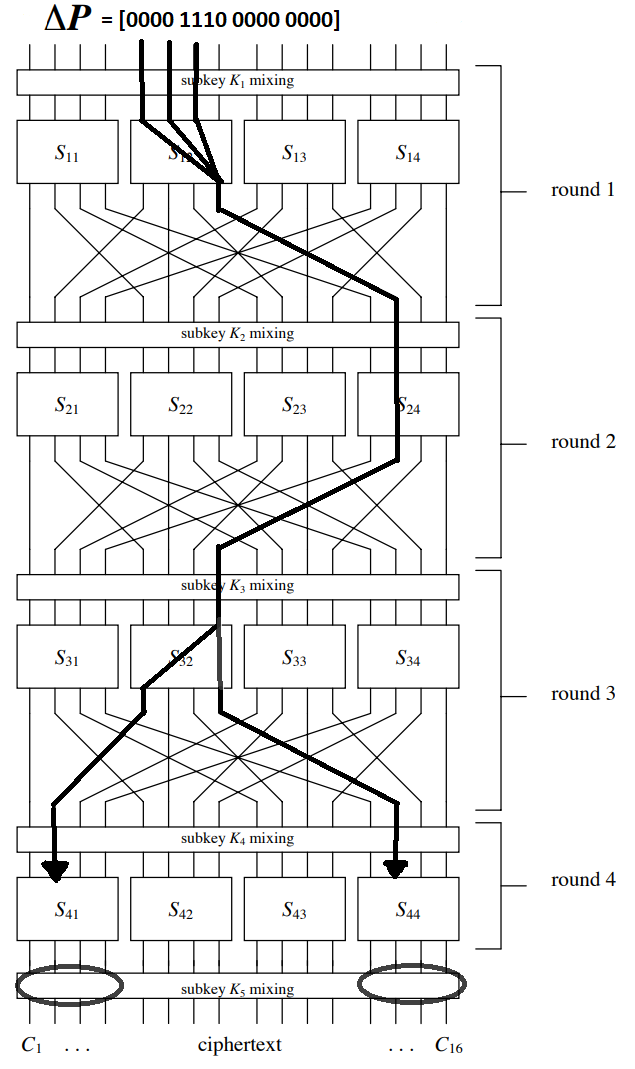
\includegraphics[width=300px]{SPN-Differential}
\centering

\noindent

On obtient la différentielle intermédiaire suivante $\boxed{\Delta I = \text{ 0100 0000 0000 0100}}$
\end{document}
